\documentclass[10pt, compress]{beamer}  
\usetheme{metropolis}
%\usepackage{setspace} %this broke footnotes
\usepackage{epstopdf,amsmath,amsfonts,amssymb,amsthm}
\usepackage{jf}
\usepackage{hyperref}
%\usepackage[margin=1.0in]{geometry}
%\usepackage{placeins}
\usepackage{rotating}
%\usepackage[utf8]{inputenc}
\usepackage{booktabs}
\usepackage{pifont}
%\usepackage{tikz}
\usepackage{pgfplots}
\usepgfplotslibrary{dateplot}
\usepackage{tikzscale}
\usepgfplotslibrary{fillbetween}
%\usepackage[flushleft]{threeparttable}

\usepackage[most]{tcolorbox}% http://ctan.org/pkg/tcolorbox           
\usepackage[normalem]{ulem}                
\usepackage[scale=2]{ccicons}                 
\usepackage[super]{nth}                 
\usepackage{lmodern}
\newcommand{\semitransp}[2][35]{\color{fg!#1}#2}

%\usepackage{natbib}
%\bibliographystyle{jf}  
\usepackage[natbib, authordate, strict, backend=bibtex8, doi=only]{biblatex-chicago}
\addbibresource{sub/capacitybib.bib}
\usepackage{graphicx}
\usepackage[labelfont=bf,labelsep=period]{caption}   % Format figure 
\captionsetup[table]{labelsep=none}

\graphicspath{{.}{./sub/fig}}

%%%%%%%%Uncomment if making printable version for standout correction%%%%%%%
%\setbeamercolor{palette primary}{fg=black, bg=white}

\renewcommand\textbullet{\ensuremath{\bullet}}                  
\setbeamertemplate{bibliography item}{}           


\newcommand{\ctabtitle}[1]{\caption[#1]{\\ \textbf{#1}}}
\newcommand{\ctabsubtitle}[1]{\caption[#1]{\; \textit{#1}}}
\newcommand{\ctabnote}[1]{\begin{flushleft} #1 \end{flushleft}}

\newcommand{\cfigcaption}[2]{\caption[#1]{\textbf{\\#1} \\ #2}}
\newcommand{\cfigtitle}[1]{\caption[#1]{ \\ \textbf{#1} }}
\newcommand{\cfigbeamcaption}[1]{\caption*{\\ #1}}

%Chernov Method
%1) What is the problem?
%2) WHy is it important?
%3) How are you solving the problem?
%4) Results

%%%%%%%%%%%%%Kicker boxes
\definecolor{zaffre}{rgb}{0.0, 0.08, 0.66}
\newtcolorbox{kicker}{colback=zaffre,arc=0.5mm,coltext=white, fontupper=\bfseries, colframe=black, halign=flush left, left=0.75mm, top=0.75mm, bottom=0.75mm, right=0.75mm}

\definecolor{mgrey}{rgb}{0.2824,0.3176,0.298}
\definecolor{lgrey}{rgb}{.7176, .7451, .7333}
\definecolor{vlgrey}{rgb}{.9098, .9176, .9137}
\newtcolorbox{quotebox}[1]{colback=vlgrey,
colframe=mgrey,fonttitle=\bfseries,
title=#1, left=1mm, top=1mm, bottom=1mm, right=1mm}
%%%%%%%%%%%%%%%%%%%%%%%
%Variable fonts per slide
%https://tex.stackexchange.com/questions/33969/changing-font-size-of-selected-slides-in-beamer
\usepackage{environ}
\usepackage{lipsum}

%
% Custom font for a frame.
%
\newcommand{\customframefont}[1]{
\setbeamertemplate{itemize/enumerate body begin}{#1}
\setbeamertemplate{itemize/enumerate subbody begin}{#1}
}

\NewEnviron{framefont}[1]{
\customframefont{#1} % for itemize/enumerate
{#1 % For the text outside itemize/enumerate
\BODY
}
\customframefont{\normalsize}
}

\setbeamercolor{background canvas}{bg=white}
%%%%%%%%%%%%%%%%%%%%%%%%%%%%%


%Some stuff from a previous document, not totallly sure what this is
\setbeamertemplate{blocks}[rounded][shadow=true]                  
\metroset{block=fill}                 
\definecolor{mycolor}{rgb}{0.122, 0.435, 0.698}% Rule colour
\makeatletter


\makeatother
%\author[Tepper]{Clinton Tepper\inst{\text{\ding{169}}}}
%\institute[]{\inst{\text{\ding{169}}} UCLA Anderson School of Management}
\author[Tepper]{iCapital Portfolio Analytics}
\title{\Large \bf GMAM 3.0}

\date{\today}

\begin{document}

\newcommand{\tstar}{\ensuremath{^\text{***}}}
\newcommand{\dstar}{\ensuremath{^\text{**}}}
\newcommand{\ostar}{\ensuremath{^\text{*}}}
\maketitle

%%%%%%%%%%%%%%%%%%%%%%%%%%%%%%%%%%%


\begin{frame}[fragile]
\frametitle{The Research Process}
\begin{figure}
	\centering
	%\includegraphics[width=0.95\linewidth]{sub/fig/paxsectionalverification-mfs.pdf}
	%\includegraphics[width=0.95\linewidth]{sub/fig/xmomassetsfs.tikz}
	\includegraphics[width=1.04\linewidth]{docs/theory/Model Development.pdf}\\
    \bigskip
\end{figure}

\end{frame}


\begin{frame}[fragile]
\frametitle{Mean Field Variational Bayes: Motivation} \label{fr:motivation}
\begin{itemize}
    \item Frequentist methods fix the parameters in the data-generating process (DGP) and assume the data is generated randomly.
    \item []
    \item Bayesian methods invert the DGP by fixing the data and inferring the likely distribution of parameters.
    \item []
    \item Bayesian estimators are admissible in the statistical sense: given the data generating process and a loss function, no other estimator always performs better (weakly dominates) the Bayesian estimator.
    \item []
    \item Drawbacks: priors (sometimes), tractability, and performance.
\end{itemize}
\end{frame}

\begin{frame}[fragile]
\frametitle{Mean Field Variational Bayes: Motivation} \label{fr:motivation}
\begin{itemize}
    \item Priors influence the results, but they also serve as a convenient and statistically rigorous approach for incorporating outside information (e.g. cross-sectional data) into the estimates.
    \item []
    \item Tractability issues stem from what is also Bayesian model's greatest strength: every unknown parameter is viewed probabilistically with respect to the values it could take given fixed observations.
    \item []
    \item Performance issues are specific to the solution methodology, but the most common (MCMC) requires extensive simulation in the estimation process
    
    \item []
    \vspace{12pt}
    \begin{kicker}
        The Mean Field Variational Bayes (MFVB) likely provides a tractable high performance solution.
    \end{kicker}
\end{itemize}
\end{frame}


\begin{frame}[fragile]
\frametitle{GMAM 3.0}
\begin{figure}
	\centering
	%\includegraphics[width=0.95\linewidth]{sub/fig/paxsectionalverification-mfs.pdf}
	%\includegraphics[width=0.95\linewidth]{sub/fig/xmomassetsfs.tikz}
	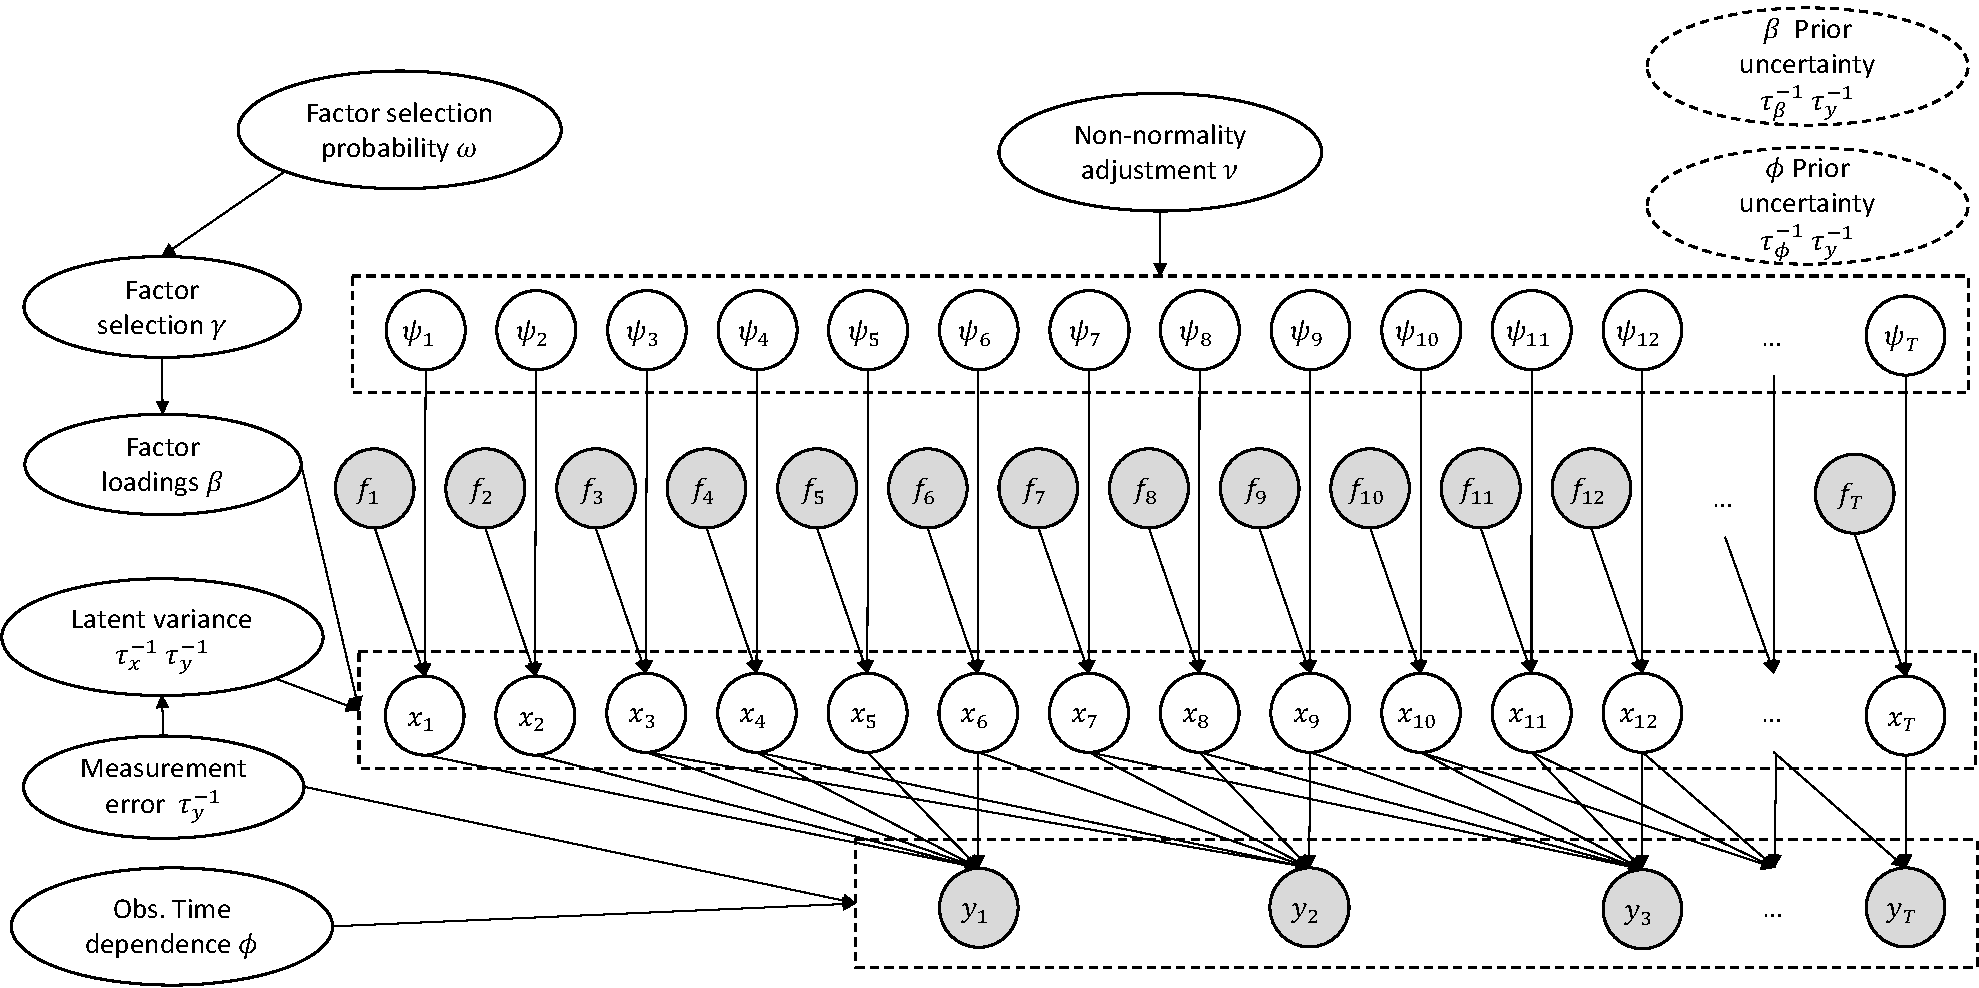
\includegraphics[width=1.04\linewidth]{docs/theory/DAG.pdf}\\
    \bigskip
    \begin{kicker}
        The hierarchical structure of GMAM 3.0 provides a flexible and rigorous statistical framework for advanced portfolio analytics.
    \end{kicker}
\end{figure}

\end{frame}

\begin{frame}[fragile]
\frametitle{Mean Field Variational Bayes: MCMC}
\begin{itemize}
    \item Markov Chain Monte Carlo (MCMC) is a highly flexible procedure for computing the distribution of parameter estimates given the data.
    \item []
    \item In infinite time and mild regularity conditions, MCMC provides the EXACT distribution of the posterior.
    \item []
    \item But...it ranges from slow (Gibbs sampling with conjugate priors) to very slow (Metropolis-Hastings, other samplers).
    \begin{itemize}
        \item A typical MCMC chain will draw from the conditional distributions well over a $100,000$ times. 
        \item For a model of the complexity of GMAM 3.0, that equates to tens of millions of random draws, each using different distributional parameters.
        \item Smaller quantities of draws are possible, but would need careful testing of efficacy.
    \end{itemize}
\end{itemize}
\end{frame}


\begin{frame}[fragile]
\frametitle{Mean Field Variational Bayes: MCMC}
\begin{itemize}
    \item Consider a simple MCMC:
    \begin{align}
        \mu_i &\sim p\left(\mu | \sigma^2_{i-1},D\right)\\
        \sigma^2_i &\sim p\left(\sigma^2 | \mu_i,D\right)
    \end{align}
    \item Because the probability distributions are conditional, sequential numerical simulation is necessary to analyze the marginal
    \item []
    \item Variational Bayesian (VB) techniques provide an alternative approach.
\end{itemize}
\end{frame}



\begin{frame}[fragile]
\frametitle{Mean Field Variational Bayes: Basic Idea}
\begin{itemize}
    \item The full posterior of the previously described problem is given by:
    \begin{align*}
        \mu,\sigma^2 \sim p(\mu,\sigma^2|D)
    \end{align*}
    \item []
    \item Suppose the posterior factored as follows:
    \begin{align*}
        p(\mu,\sigma^2|D)&\propto q_\mu(\mu)q_{\sigma^2}(\sigma^2) 
    \end{align*}
    \item []
    \item Then the econometrician could simply compute summary statistics on $q_\mu(\mu)$ and  $q_{\sigma^2}(\sigma^2)$.
\end{itemize}
\end{frame}

\begin{frame}[fragile]
\frametitle{Mean Field Variational Bayes: Basic Idea}
\begin{itemize}
    \item Importantly, the posterior does NOT factor this way. 
    \item []
    \item VB is an approximation, the goal of which is to find the distribution $q(\cdot)$ which maximizes the accuracy of the approximation.
    \item []
    \item In the variant employed in GMAM 3.0, $q(\cdot)$ is selected to minimize the KL divergence between the approximating distribution and the true (conditional) posterior.
\end{itemize}
\end{frame}

\begin{frame}[fragile]
\frametitle{Mean Field Variational Bayes: Application to GMAM 3.0}

The VB approximation to GMAM 3.0:
\begin{align*}
    p\left(\Theta|D\right)&\underset{\sim}{\propto}q\left(\phi\right)\times q\left(\tau_{y}\right)\times q\left(x\right)\\
    &\times q\left(\beta\right)\times q\left(\tau_{x}\right)\times\prod_{t\in1:T}q\left(\psi_{i}\right)\\
    &\times q\left(\nu\right)\times\prod_{k\in1:K}q\left(\gamma_{k}\right)\times q\left(\omega\right)
\end{align*}

\begin{table}
\scriptsize

%\caption{\bf\scriptsize \;Explanatory volume regressions (1 month, 18-month rolling)}
\vspace{-10pt}   
    \begin{tabular}{ccl}
    \toprule 
        Variable & Type & Definition/Description\tabularnewline
        \midrule
            $x$ & Local & $x$ is a vector of latent economic returns\tabularnewline
            $\phi$ & Local & $\phi$ is the moving average window\tabularnewline
            $\tau_{y}$ & Global & Precision parameter for independent measurement error\tabularnewline
            $\beta$ & Local & Regression coefficients of $x$ on $F$\tabularnewline
            $\psi$ & Local & $\psi$ is a vector of precision weights for $x$\tabularnewline
            $\tau_{x}$ & Global & Precision parameter for the regression of $x$ on $F$\tabularnewline
            $\gamma$ & Local & Vector of variable selection indicators\tabularnewline
            $\omega$ & Global & Probability of variable selection\tabularnewline
            $\nu$ & Global & Non-normality parameter for $x$; DOF of posterior $t$ distribution\tabularnewline
        \bottomrule
    \end{tabular}
\end{table}
\end{frame}



\begin{frame}[fragile]
\frametitle{GMAM 3.0: The plan}
\begin{figure}
	\centering
	%\includegraphics[width=0.95\linewidth]{sub/fig/paxsectionalverification-mfs.pdf}
	%\includegraphics[width=0.95\linewidth]{sub/fig/xmomassetsfs.tikz}
	\includegraphics[width=1.02\linewidth]{docs/theory/PERT.pdf}\\
    \bigskip
    \raggedright{
     Note: While the dependencies are strict (except for \#6), the process is highly iterative: earlier steps will need rework based on findings in later steps.}
\end{figure}
\end{frame}

\begin{frame}[fragile]
\frametitle{GMAM 3.0: The plan}
\begin{enumerate}
    \item Model the DGP in terms of observed data and unobserved parameters
    \item Assign prior distributions (usually conjugate)
    \item Derive conditional posterior distributions
    \item Derive approximating VB distributions
    \item For each parameter, verify the conditional posterior and approximating VB distributions via numerical simulation
    \item Determine a strategy for computing prior hyper parameters
    \item Construct an MCMC for the conditional posterior distributions
    \item Estimate the VB system and compare the accuracy to the MCMC results
\end{enumerate}
\end{frame}

\end{document}